%\documentclass[handout]{beamer}
\documentclass[compress]{beamer}
\usepackage[T1]{fontenc}
\usepackage{pifont}
\usetheme[block=fill,subsectionpage=progressbar,sectionpage=progressbar]{metropolis} 

\usepackage{minted}

\usepackage{hyperref}
\hypersetup{ %
	pdfborder = {0 0 0},
	colorlinks=true,
}


\definecolor{Purple}{HTML}{911146}
\definecolor{Orange}{HTML}{CF4A30}

% Theme colors are derived from these two elements
\setbeamercolor{alerted text}{fg=Orange}

% ... however you can of course override styles of all elements
\setbeamercolor{frametitle}{bg=Purple}


\usepackage{wasysym}
\usepackage{etoolbox}
\usepackage[utf8]{inputenc}

\usepackage{threeparttable}
\usepackage{subcaption}

\usepackage{tikz-qtree}
\setbeamercovered{still covered={\opaqueness<1->{5}},again covered={\opaqueness<1->{100}}}





\usepackage{listings}

\lstset{
	basicstyle=\scriptsize\ttfamily,
	columns=flexible,
	breaklines=true,
	numbers=left,
	%stepsize=1,
	numberstyle=\tiny,
	backgroundcolor=\color[rgb]{0.85,0.90,1}
}



\lstnewenvironment{lstlistingoutput}{\lstset{basicstyle=\footnotesize\ttfamily,
		columns=flexible,
		breaklines=true,
		numbers=left,
		%stepsize=1,
		numberstyle=\tiny,
		backgroundcolor=\color[rgb]{.7,.7,.7}}}{}


\lstnewenvironment{lstlistingoutputtiny}{\lstset{basicstyle=\tiny\ttfamily,
		columns=flexible,
		breaklines=true,
		numbers=left,
		%stepsize=1,
		numberstyle=\tiny,
		backgroundcolor=\color[rgb]{.7,.7,.7}}}{}


\usepackage[american]{babel}
\usepackage{csquotes}

\usepackage[natbib=true,style=authoryear,backend=bibtex,useprefix=true]{biblatex}
\addbibresource{../literature.bib}

\renewcommand*{\bibfont}{\tiny}

\usepackage{tikz}
\usetikzlibrary{shapes,arrows,matrix}
\usepackage{multicol}

\usepackage{subcaption}

\usepackage{booktabs}
\usepackage{graphicx}

\graphicspath{{../pictures/}}

\makeatletter
\setbeamertemplate{headline}{%
	\begin{beamercolorbox}[colsep=1.5pt]{upper separation line head}
	\end{beamercolorbox}
	\begin{beamercolorbox}{section in head/foot}
		\vskip2pt\insertnavigation{\paperwidth}\vskip2pt
	\end{beamercolorbox}%
	\begin{beamercolorbox}[colsep=1.5pt]{lower separation line head}
	\end{beamercolorbox}
}
\makeatother



\setbeamercolor{section in head/foot}{fg=normal text.bg, bg=structure.fg}



\newcommand{\question}[1]{
	\begin{frame}[plain]
		\begin{columns}
			\column{.4\textwidth}
			\makebox[\columnwidth]{
				
\includegraphics[width=\columnwidth,height=\paperheight,keepaspectratio]{../pictures/mannetje.png}}
			\column{.6\textwidth}
			\large
			\textcolor{orange}{\textbf{\emph{#1}}}
		\end{columns}
\end{frame}}

\newcommand{\instruction}[1]{\emph{\textcolor{gray}{[#1]}}}


\title[Computational Communication Science 2]{\textbf{Computational Communication Science 2} \\Week 2 - Lecture\\ »Text as Data «}
\author[Anne Kroon]{Anne Kroon \\ ~ \\ \footnotesize{ a.c.kroon@uva.nl, @annekroon} \\}
\date{April, 2022}
\institute[Digital Society Minor, University of Amsterdam]{Digital Society Minor, University of Amsterdam}

\begin{document}
	
	\begin{frame}{}
		\titlepage
	\end{frame}
	
	\begin{frame}{Today}
		\begin{tiny}
		\tableofcontents
		\end{tiny}
	\end{frame}


\section{The toolkit}

\subsection{Bottom-up vs. top-down}

\begin{frame}[standout]
	Automated content analysis can be either \textcolor{red}{bottom-up} (inductive, explorative, pattern recognition, \ldots) or \textcolor{red}{top-down} (deductive, based on a-priori developed rules, \ldots). Or in between.
\end{frame}


\begin{frame}{The CCS toolbox}
	\makebox[\columnwidth]{
		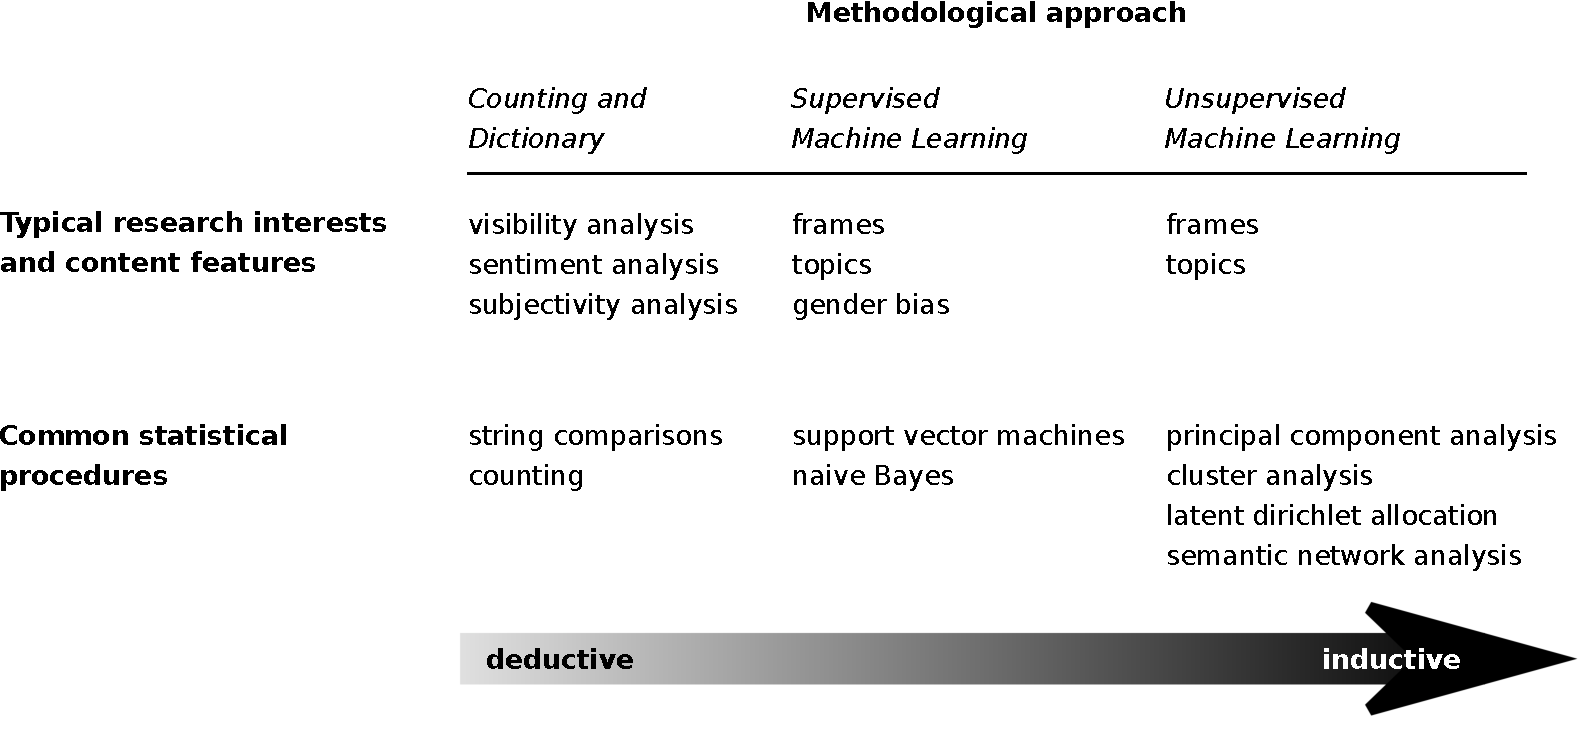
\includegraphics[width=\columnwidth,height=\paperheight,keepaspectratio]{../pictures/boumanstrilling2016}}
	\\
	\cite{Boumans2016}
\end{frame}

\begin{frame}{Bottom-up vs. top-down}
	\begin{block}{Bottom-up}
		\begin{itemize}
			\item Count most frequently occurring words 
			\item Maybe better: Count combinations of words $\Rightarrow$ Which words co-occur together?
		\end{itemize}
		We \emph{don't} specify what to look for in advance	
	\end{block}
	
	\onslide<2>{
		\begin{block}{Top-down}
			\begin{itemize}
				\item Count frequencies of pre-defined words
				\item Maybe better: patterns instead of words
			\end{itemize}
			We \emph{do} specify what to look for in advance	
		\end{block}
	}
\end{frame}


\begin{frame}[fragile]{A simple bottom-up approach}

\begin{minted}[%
	breaklines,
	linenos,
	fontsize=\scriptsize,
	frame=single,
	xleftmargin=0pt,]
	{python}
from collections import Counter
texts = ["Communication in the Digital Society is a very very complex phenomenon", "I like to study it"]
bottom_up = []
for t in texts:
    bottom_up.append(Counter(t.lower().split()).most_common(3))
print(bottom_up)
\end{minted}
\pause
This results in:
\begin{minted}[fontsize=\scriptsize]{python}
[('very', 2), ('Communication', 1), ('in', 1)]
[('I', 1), ('like', 1), ('to', 1)]
\end{minted}
\textcolor{red}{\footnotesize{\emph{Please note that you can also write this like:}}}
\pause
\begin{minted}[%
	breaklines,
	linenos,
	fontsize=\scriptsize,
	frame=single,
	xleftmargin=0pt,]
	{python}
bottom_up = [Counter(t.split()).most_common(3) for t  in texts]
\end{minted}
\begin{itemize}
\tiny{
	\item This is \emph{exactly} the same, just shorter (and faster). 
	\item You do \emph{not} have to use list comprehensions, but it helps if you can read them. }
\end{itemize}

\end{frame}

\begin{frame}[fragile]{A simple top-down approach}
\begin{minted}[%
	breaklines,
	linenos,
	fontsize=\scriptsize,
	frame=single,
	xleftmargin=0pt,]
	{python}
texts = ["Communication in the Digital Society is a very very complex phenomenon", "I like to study it"]
features = ["communication", "digital", "study"]
for t in texts:
    print(f"\nAnalyzing '{t}':")
       for f in features:
          print(f"{f} occurs {t.lower().count(f)} times")
\end{minted}
\pause
\begin{minted}[fontsize=\tiny]{python}
Analyzing 'Communication in the Digital Society is a very very complex phenomenon':
communication occurs 1 times
digital occurs 1 times
study occurs 0 times

Analyzing 'I like to study it':
communication occurs 0 times
digital occurs 0 times
study occurs 1 times	
\end{minted}
\pause
\textcolor{red}{\footnotesize{\emph{\dots save the results as a \texttt{list} as follows \dots}}}
\pause
\begin{minted}[%
	breaklines,
	linenos,
	fontsize=\tiny,
	frame=single,
	xleftmargin=0pt,]
	{python}
top_down = [[t.lower().count(f) for f in features] for t in texts]
\end{minted}
\end{frame}

\question{When would you use which approach?}


\begin{frame}{Some considerations}
	\begin{itemize}[<+->]
		\item Both can have a place in your workflow (e.g., bottom-up as first exploratory step)
		\item You have a clear theoretical expectation? Bottom-up makes little sense.
		\item But in any case: you need to transform your text into something ``countable''.
	\end{itemize}
\end{frame}


\subsection{Approaches to working with text}

\begin{frame}{The toolbox}
	\begin{block}{Slicing}
		\texttt{mystring[2:5]} to get the characters with indices 2,3,4
	\end{block}
	
	\begin{block}{String methods}
		\begin{itemize}
			\item \texttt{.lower()} returns lowercased string
			\item \texttt{.strip()} returns string without whitespace at beginning and end
			\item \texttt{.find("bla")} returns index of position of substring ``bla'' or -1 if not found
			\item \texttt{.replace("a","b")} returns string where "a" is replaced by "b"
			\item \texttt{.count("bla")} counts how often substring ``bla'' occurs
		\end{itemize}
		Use tab completion for more!
	\end{block}
\end{frame}

\section{Natural Language Processing}
\begin{frame}
	Natural Language Processing
\end{frame}

\begin{frame}{NLP: What and why?}
	\begin{block}{Preprocessing steps}
		\begin{description}
			\item [tokenization] How do we (best) split a sentence into tokens (terms, words)?
			\item [pruning] How can we remove unneccessary words/ punctuation?
			\item [lemmatization] How can we make sure that slight variations of the same word are not counted differently?
		\end{description}
	\end{block}
\end{frame}


\subsection{Better tokenization}

\begin{frame}[fragile]{OK, good enough, perfect?}
	\begin{block}{.split()}
		\begin{itemize}
			\item space $\rightarrow$ new word
			\item no further processing whatsoever
			\item thus, only works well if we do a preprocessing outselves (e.g., remove punctuation)
		\end{itemize}
	\end{block}
\pause
\begin{minted}[%
	breaklines,
	linenos,
	fontsize=\scriptsize,
	frame=single,
	xleftmargin=0pt,]
	{python}
docs = ["This is a text",  "I haven't seen John's derring-do. Second sentence!"]
tokens = [d.split() for d in docs]
\end{minted}
	
\begin{minted}[%
	fontsize=\scriptsize,]
	{python}
[['This', 'is', 'a', 'text'], ['I', "haven't", 'seen', "John's", 'derring-do.', 'Second', 'sentence!']]
\end{minted}
\end{frame}


\begin{frame}[fragile]{OK, good enough, perfect?}
	\begin{block}{Tokenizers from the NLTK package}
		\begin{itemize}
			\item multiple improved tokenizers that can be used instead of .split()
			\item e.g., Treebank tokenizer:
			\begin{itemize}
				\item split standard contractions ("don't")
				\item deals with punctuation
			\end{itemize}			
		\end{itemize}
	\end{block}
\pause
\begin{minted}[%
	breaklines,
	linenos,
	fontsize=\scriptsize,
	frame=single,
	xleftmargin=0pt,]
	{python}
from nltk.tokenize import TreebankWordTokenizer
tokens = [TreebankWordTokenizer().tokenize(d) for d in docs]
\end{minted}
\pause
\begin{minted}[%
breaklines,
fontsize=\scriptsize]
{python}
[['This', 'is', 'a', 'text'],  ['I', 'have', "n't", 'seen', 'John', "'s", 'derring-do.', 'Second', 'sentence', '!']]
\end{minted}
\tiny{Notice the failure to split the \texttt{.} at the end of the first sentence in the second doc. That's because \texttt{TreebankWordTokenizer} expects \emph{sentences} as input. See book for a solution.\\}
\end{frame}


\subsection{Stopword and punctuation removal}

\begin{frame}
	\textbf{Stopword removal} \\
	\vspace{1cm}
	\begin{itemize}
		\item <2->{\emph{The logic of the algorithm is very much related to the one of a simple sentiment analysis!}}
	\end{itemize}
\end{frame}

\begin{frame}{Stopword removal}
	\begin{block}{What are stopwords?}
		\begin{itemize}
			\item Very frequent words with little inherent meaning
			\item \texttt{the, a, he, she, \ldots}
			\item context-dependent: if you are interested in gender, \texttt{he} and \texttt{she} are no stopwords. 
			\item Many existing lists as basis
		\end{itemize}
	\end{block}
	
\end{frame}

\begin{frame}{Stopword removal: What and why?}
	\begin{block}{Why remove stopwords?}
		\begin{itemize}
			\item If we want to identify key terms (e.g., by means of a word count), we are not interested in them
			\item If we want to calculate document similarity, it might be inflated
			\item If we want to make a word co-occurance graph, irrelevant information will dominate the picture
		\end{itemize}
	\end{block}
\end{frame}

\begin{frame}[fragile]{Stopword removal}
\begin{minted}[%
	breaklines,
	linenos,
	fontsize=\scriptsize,
	frame=single,
	xleftmargin=0pt,]
	{python}
from nltk.corpus import stopwords
mystopwords = stopwords.words("english")
mystopwords.extend(["test", "this"])

tokens_without_stopwords = [[word for word in doc if word.lower() not in mystopwords] for doc in tokens]
\end{minted}
\begin{minted}[%
fontsize=\scriptsize,]
{python}
[['text'], ["n't", 'seen', 'John', 'derring-do.', 'Second', 'sentence', '!']]
\end{minted}
	
\begin{alertblock}{You can do more!}
		\tiny{For instance, in line 8, you could add an \texttt{or} statement to also exclude punctuation.}
\end{alertblock}
	
\end{frame}


\begin{frame}[fragile]{Removing punctuation}
\begin{minted}[%
	breaklines,
	linenos,
	fontsize=\scriptsize,
	frame=single,
	xleftmargin=0pt,]
	{python}
from nltk.tokenize import RegexpTokenizer
tokenizer = RegexpTokenizer(r'\w+')
tokenizer.tokenize("Hi students, what's up!")
\end{minted}
\pause
\begin{minted}[%
	fontsize=\scriptsize,]
	{python}
['Hi', 'students', 'what', 's', 'up']
\end{minted}	
\end{frame}


\subsection{ngrams}
\begin{frame}
	Instead of just looking at single words (unigrams), we can also use adjacent words (bigrams).
\end{frame}

\begin{frame}[fragile]{ngrams}
\begin{minted}[%
	breaklines,
	linenos,
	fontsize=\scriptsize,
	frame=single,
	xleftmargin=0pt,]
	{python}
import nltk
texts = ['This is the first text text text first', 'And another text yeah yeah']
texts_bigrams = [["_".join(tup) for tup in nltk.ngrams(t.split(),2)] for t in texts]
print(texts_bigrams)
\end{minted}

	\texttt{[['This\_is',
		'is\_the',
		'the\_first',
		'first\_text',
		'text\_text',
		'text\_text',
		'text\_first'],
		['And\_another', 'another\_text', 'text\_yeah', 'yeah\_yeah']]
	}

Typically, we would combine both.
	\pause
	\textbf{\textcolor{red}{What do you think? Why is this useful? (and what may be drawbacks?)}}
\end{frame}


\begin{frame}{Main takeaway}
	
	\begin{itemize}
		%	\item It matters how you transform your text into numbers (``vectorization'').
		\item Preprocessing matters, be able to make informed choices.
		\item Keep this in mind when moving to Machine Learning. 
	\end{itemize}
\end{frame}


\section{From text to features: vectorizers}

\subsection{General idea}

\begin{frame}[fragile]{A text as a collections of word}
	
	Let us represent a string 
\begin{minted}[%
	breaklines,
	linenos,
	fontsize=\scriptsize,
	frame=single,
	xleftmargin=0pt,]
	{python}
t = "This this is is is a test test test"
# like this:
print(Counter(t.split()))
\end{minted}
\begin{minted}[%
	breaklines,
	fontsize=\scriptsize,]
	{python}
Counter({'is': 3, 'test': 3, 'This': 1, 'this': 1, 'a': 1})
\end{minted}
	
	\pause 
	Compared to the original string, this representation
	\begin{itemize}
		\item is less repetitive
		\item preserves word frequencies
		\item but does \emph{not} preserve word order
		\item can be interpreted as a vector to calculate with (!!!)
	\end{itemize}
	
	\tiny{\emph{Of course, still a lot of stuff to fine-tune\ldots}  (for example, This/this)}
\end{frame}



\begin{frame}{From vector to matrix}
	If we do this for multiple texts, we can arrange the vectors in a table.
	
	t1 = "This this is is is a test test test" \newline
	t2 = "This is an example"
	
	\begin{tabular}{| c|c|c|c|c|c|c|c|}
		\hline
		& a & an & example & is & this & This & test \\
		\hline
		\emph{t1} & 1 & 0 & 0 & 3 & 1 & 1 & 3 \\
		\emph{t2} &0 & 1 & 1 & 1 & 0 & 1 & 0 \\
		\hline
	\end{tabular}
\end{frame}


\question{What can you do with such a matrix? Why would you want to represent a collection of texts in such a way?}

\begin{frame}{What is a vectorizer}
	\begin{itemize}[<+->]
		\item Transforms a list of texts into a sparse (!) matrix (of word frequencies)
		\item Vectorizer needs to be ``fitted'' to the training data (learn which words (features) exist in the dataset and assign them to columns in the matrix)
		\item Vectorizer can then be re-used to transform other datasets 
	\end{itemize}
\end{frame}


\begin{frame}{The cell entries: raw counts versus tf$\cdot$idf scores}
	\begin{itemize}
		\item In the example, we entered simple counts (the ``term frequency'')
	\end{itemize}
\end{frame}

\question{But are all terms equally important?}


\begin{frame}{The cell entries: raw counts versus tf$\cdot$idf scores}
	\begin{itemize}
		\item In the example, we entered simple counts (the ``term frequency'')
		\item But does a word that occurs in almost all documents contain much information?
		\item And isn't the presence of a word that occurs in very few documents a pretty strong hint?
		\item<2-> \textbf{Solution: Weigh by \emph{the number of documents in which the term occurs at least once) (the ``document frequency'')}} 
	\end{itemize}
	\onslide<3->{
		$\Rightarrow$ we multiply the ``term frequency'' (tf) by the inverse document frequency (idf)
		
		\tiny{(usually with some additional logarithmic transformation and normalization applied, see \url{https://scikit-learn.org/stable/modules/generated/sklearn.feature_extraction.text.TfidfTransformer.html})}
	}
\end{frame}

\begin{frame}{tf$\cdot$idf}
	\begin{array}{ccc}
		
		w_{i, j}=t f_{i, j} \times \log \left(\frac{N}{d f_{i}}\right)  \\ \\
		
		t f_{i, j}=\text { number of occurrences of } i \text { in } j \\
		d f_{i}=\text { number of documents containing } i \\
		N=\text {total number of documents }
	\end{array}
\end{frame}

\begin{frame}{Is tf$\cdot$idf always better?}
	It depends.
	
	\begin{itemize}
		\item Ultimately, it's an empirical question which works better ($\rightarrow$ machine learning)
		\item In many scenarios,  ``discounting'' too frequent words and ``boosting'' rare words makes a lot of sense (most frequent words in a text can be highly un-informative)
		\item Beauty of raw tf counts, though: interpretability + describes document in itself, not in relation to other documents
	\end{itemize}
\end{frame}


\begin{frame}{Different vectorizers}
	\begin{enumerate}[<+->]
		\item CountVectorizer (=simple word counts)
		\item TfidfVectorizer (word counts (``term frequency'') weighted by number of documents in which the word occurs at all (``inverse document frequency''))
	\end{enumerate}
\end{frame}

\begin{frame}{Internal representations}
	\begin{block}{Sparse vs dense matrices}
		\begin{itemize}
			\item $\rightarrow$ tens of thousands of columns (terms), and one row per document
			\item Filling all cells is inefficient \emph{and} can make the matrix too large to fit in memory (!!!)
			\item Solution: store only non-zero values with their coordinates! (sparse matrix)
			\item dense matrix (or dataframes) not advisable, only for toy examples
		\end{itemize}
	\end{block}
\end{frame}


{\setbeamercolor{background canvas}{bg=black}
	\begin{frame}
		\makebox[\linewidth]{
			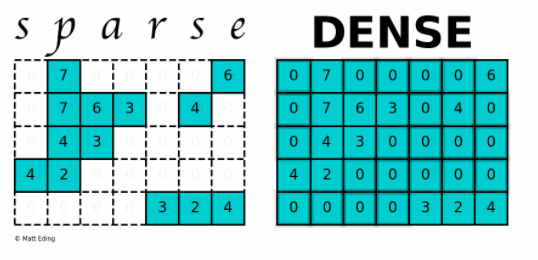
\includegraphics[width=\paperwidth,height=\paperheight,keepaspectratio]{../pictures/sparse_dense.png}}
		\url{https://matteding.github.io/2019/04/25/sparse-matrices/}
	\end{frame}
}


\begin{frame}[standout]
We justed learned how to tokenize with a list comprehension (and that's often a good idea!). But what if we want to \emph{directly} get a DTM instead of lists of tokens?
\end{frame}


\begin{frame}[fragile]{OK, good enough, perfect?}
	\begin{block}{scikit-learn's CountVectorizer (default settings)}
		\begin{itemize}
			\item applies lowercasing
			\item deals with punctuation etc. itself
			\item minimum word length $>1$
			\item more technically, tokenizes using this regular expression: \texttt{r"(?u)\textbackslash b\textbackslash w\textbackslash w+\textbackslash b"} \footnote{?u = support unicode, \textbackslash b = word boundary}
		\end{itemize}
	\end{block}
\begin{minted}[%
	breaklines,
	linenos,
	fontsize=\scriptsize,
	frame=single,
	xleftmargin=0pt,]
	{python}
from sklearn.feature_extraction.text import CountVectorizer
cv = CountVectorizer()
dtm_sparse = cv.fit_transform(docs)
\end{minted}
\end{frame}


\begin{frame}{OK, good enough, perfect?}
	\begin{block}{CountVectorizer supports more}
		\begin{itemize}
			\item stopword removal
			\item custom regular expression
			\item or even using an external tokenizer
			\item ngrams instead of unigrams
		\end{itemize}
	\end{block}
	\tiny{see \url{https://scikit-learn.org/stable/modules/generated/sklearn.feature\_extraction.text.CountVectorizer.html}}
	
	\pause
	\begin{alertblock}{Best of both worlds}
		\textbf{Use the Count vectorizer with a NLTK-based external tokenizer! (see book)}
	\end{alertblock}
\end{frame}


\subsection{Pruning}

\begin{frame}{General idea}
	\begin{itemize}
		\item Idea behind both stopword removal and tf$\cdot$idf: too frequent words are uninformative
		\item<2-> (possible) downside stopword removal: a priori list, does not take empirical frequencies in dataset into account
		\item<3-> (possible) downside tf$\cdot$idf: does not reduce number of features
	\end{itemize}
	
	\onslide<4->{Pruning: remove all features (tokens) that occur in less than X or more than X of the documents}
\end{frame}

\begin{frame}[fragile, plain]
	CountVectorizer, only stopword removal
\begin{minted}[%
	breaklines,
	linenos,
	fontsize=\tiny,
	frame=single,
	xleftmargin=0pt,]
	{python}
from sklearn.feature_extraction.text import CountVectorizer, TfidfVectorizer
myvectorizer = CountVectorizer(stop_words=mystopwords)
\end{minted}
CountVectorizer, better tokenization, stopword removal (pay attention that stopword list uses same tokenization!):
\begin{minted}[%
	breaklines,
	linenos,
	fontsize=\tiny,
	frame=single,
	xleftmargin=0pt,]
	{python}
myvectorizer = CountVectorizer(tokenizer = TreebankWordTokenizer().tokenize, stop_words=mystopwords)
\end{minted}
	
	Additionally remove words that occur in more than 75\% or less than $n=2$ documents:
\begin{minted}[%
	breaklines,
	linenos,
	fontsize=\tiny,
	frame=single,
	xleftmargin=0pt,]
	{python}
myvectorizer = CountVectorizer(tokenizer = TreebankWordTokenizer().tokenize, stop_words=mystopwords, max_df=.75, min_df=2)
\end{minted}
	
	All togehter: tf$\cdot$idf, explicit stopword removal, pruning
\begin{minted}[%
	breaklines,
	linenos,
	fontsize=\tiny,
	frame=single,
	xleftmargin=0pt,]
	{python}
myvectorizer = TfidfVectorizer(tokenizer = TreebankWordTokenizer().tokenize, stop_words=mystopwords, max_df=.75, min_df=2)
\end{minted}
	
	
\end{frame}


\question{What is ``best''? Which (combination of) techniques to use, and how to decide?}



\section{From test to large-scale}

\begin{frame}[fragile]{General approach}
1. Take a single string and test your idea
\begin{minted}[%
	breaklines,
	linenos,
	fontsize=\scriptsize,
	frame=single,
	xleftmargin=0pt,]
	{python}
t = "This is a test test test."
print(t.count("test"))
\end{minted}
2a. You'd assume it to return 3. If so, scale it up:
\pause
\begin{minted}[%
	breaklines,
	linenos,
	fontsize=\scriptsize,
	frame=single,
	xleftmargin=0pt,]
	{python}
results = []
for t in listwithallmytexts:
    r = t.count("test")
    print(f"{t} contains the substring {r} times")
	results.append(r)
\end{minted}

2b. If you \emph{only} need to get the list of results, a list comprehension is more elegant:
\begin{minted}[%
	breaklines,
	linenos,
	fontsize=\scriptsize,
	frame=single,
	xleftmargin=0pt,]
	{python}
results = [t.count("test") for t in listwithallmytexts]
\end{minted}


\end{frame}

\begin{frame}[fragile]{General approach}
\Large

\textcolor{red}{Test on a single string, then make a for loop or list comprehension!}

\pause

\normalsize

\begin{alertblock}{Own functions}
	If it gets more complex, you can write your ow= function and then use it in the list comprehension:
\begin{minted}[%
	breaklines,
	linenos,
	fontsize=\scriptsize,
	frame=single,
	xleftmargin=0pt,]
	{python}
def mycleanup(t):
     # do sth with string t here, create new string t2
     return t2
		
results = [mycleanup(t) for t in allmytexts]
\end{minted}
\end{alertblock}
\end{frame}


\begin{frame}[fragile]{Pandas string methods as alternative}
If you select column with strings from a pandas dataframe, pandas offers a collection of string methods (via \texttt{.str.}) that largely mirror standard Python string methods:

\begin{minted}[%
	breaklines,
	linenos,
	fontsize=\scriptsize,
	frame=single,
	xleftmargin=0pt,]
	{python}
df['newcoloumnwithresults'] = df['columnwithtext'].str.count("bla")
\end{minted}


\pause

\begin{alertblock}{To pandas or not to pandas for text?}
	Partly a matter of taste. 
	
	Not-too-large dataset with a lot of extra columns? Advanced statistical analysis planned? Sounds like pandas.
	
	It's mainly a lot of text? Wanna do some machine learning later on anyway? It's large and (potentially) messy? Doesn't sound like pandas is a good idea.
\end{alertblock}

\end{frame}



\begin{frame}{Thank you!!}
	\begin{block}{Thank you for your attention!}
		\begin{itemize}
			\item Questions? Comments?
		\end{itemize}
	\end{block}
\end{frame}



\begin{frame}
	\frametitle{References}
	\printbibliography
\end{frame}
	

\end{document}